\section{Max formulation}\label{max_formulation}

In this section will be described two methods that has been developed for the computation of the maximum of a set of random variables.
Let $X_1, X_2, ..., X_n$ be independent r.v. such that $X_i \sim N(\mu_i, \sigma_i^2)$ for every $1 \leq i \leq n.$

\subsection{Exact Method}
Let $Y = \max\{X_1, X_2, ..., X_n\}$, then
\begin{align*}
	F_Y(y) &= P_r(Y \leq y) \\
	&= P_r(\max\{X_1, X_2, ..., X_n\} \leq y) \\
	&= P_r(X_1 \leq y, X_2 \leq y, ..., X_n \leq y) \\
\end{align*}

\begin{align*}
&= \prod_{i = 1}^n P_r(X_i \leq y)  \tag*{(by indipendence of r.v)} \\
&= \prod_{i = 1}^n F_{X_i}(y)  \\
&= \prod_{i = 1}^n \Phi\left(\frac{y - \mu_i}{\sigma_i}\right) \\
\end{align*}

\begin{align*}
	f_Y(y) &= \frac{d}{dy} F_Y(y) = \frac{d}{dy} \prod_{i = 1}^n \Phi\left(\frac{y - \mu_i}{\sigma_i}\right) \\
	&= \left(\prod_{i = 1}^n \Phi\left(\frac{y - \mu_i}{\sigma_i}\right)\right) \cdot \\
	&\qquad \cdot \sum_{j = 1}^n \left(\frac{\phi\left(\frac{y - \mu_j}{\sigma_j}\right)}{\Phi\left(\frac{y - \mu_j}{\sigma_j}\right)} \cdot \frac{1}{\sigma_j}\right)
\end{align*}
where $\Phi$ is the standard normal distribution function and $\phi$ is the standard normal density function. \\
To compute the expected value, it is necessary to solve the following integral
\begin{align*}
	\mathbb{E}[Y] &= \int_{-\infty}^{+\infty} y \cdot f_Y(y)\text{ }dy \\
	&= \int_{-\infty}^{+\infty} y \cdot \left[\left(\prod_{i = 1}^n \Phi\left(\frac{y - \mu_i}{\sigma_i}\right)\right) \cdot \right. \\
	&\left. \qquad \cdot \sum_{j = 1}^n \left(\frac{\phi\left(\frac{y - \mu_j}{\sigma_j}\right)}{\Phi\left(\frac{y - \mu_j}{\sigma_j}\right)} \cdot \frac{1}{\sigma_j}\right)\right]dy
\end{align*}
that has to be computed numerically since it cannot be computed analytically.

Fixing the value of the variable $y$, the computing time for calculating $f_Y(y)$ is $\Theta(n)$, as the product operator is already computed before the sum operator. However, the majority of the computing time is consumed by the computation of the improper integral for the expected value that depends on the number of points used in the numerical integration. The number of points determines the estimated error of the result. In general, the computing time is $\theta(M n)$ where $M$ is a very large number tuned by the algorithm used for computing the integral \cite{2020SciPy-NMeth}.
Experimental results show that the function to be integrated is significantly different from zero only within a very small range of values. Estimating this range could reduce the computational cost significantly by focusing the computation on the relevant interval.

\subsection{Boost-Exact Method}
To identify a narrower integration range compared to the theoretical one, an approximate analysis of the integrand function was performed.

Specifically, it was observed that the range to be determined depends on the function \( f_Y(y) \), as the integrand function is the same but scaled by a factor \( y \), which has the role to amplify the function's value (either positively or negatively). It is worth noting that \( f_Y(y) \) is strictly positive because \( F_Y(y) \) is the product of cumulative distribution functions (whose values stay between 0 and 1), and the summation consists only of positive terms. Each term in the summation is positive since its numerator is a cumulative distribution function of a normal variable (returning a value between 0 and 1), and the denominator is always positive due to the multiplication of \( F_Y(y) \) by the standard deviation.

\subsubsection{Lower bound}
For small values of \( y \), the dominant factor that drives the value of the integrand to 0 is \( F_Y(y) \). Therefore, the goal is to determine a threshold value, referred to as the lower bound (LB), such that:
$$f_Y(y)_{|_{y = LB}} > T $$
where \( T \) is a very small number close to 0, which makes the product approach 0. An equivalent formulation of the problem is defined as follows:
\begin{align*}
    \ln{\left(\prod_{i = 1}^n \Phi\left(\frac{y - \mu_i}{\sigma_i}\right)\right)} = \\
    = \sum_{i=1}^n  \ln{\left(\Phi\left(\frac{y - \mu_i}{\sigma_i}\right)\right)}
\end{align*}
and the resulting problem is:
$$ \sum_{i=1}^n  \ln{\left(\Phi\left(\frac{y - \mu_i}{\sigma_i}\right)\right)} > \ln(T) $$
However, in general, the problem is challenging to solve analytically because the logarithmic function composed with the CDF does not have a closed form. Nevertheless, in the case where all random variables are identical, the problem can be simplified as follows:
\begin{align*}
    &n \cdot \ln{\left(\Phi\left(\frac{y - \mu}{\sigma}\right)\right)} > \ln(T) \\
    & \Rightarrow \Phi\left(\frac{y - \mu}{\sigma}\right) > e^{\ln(T) / n} \\
    & \Rightarrow y > \mu + \sigma \Phi^{-1}\left(e^{\ln(T) / n}\right)
\end{align*}
where $\Phi^{-1}$ is the Percent Point Function (PPF). To obtain an approximate solution to the general problem, it was decided to operate on the individual elements of the product as follows:
$$LB = \max_{i=0,...,n}\{\mu_i + \sigma_i \Phi^{-1}(T)\}$$
The obtained value is certainly a less accurate bound compared to the actual one.
LB ensures that each individual factor of the production function exceeds the threshold value, thereby ensuring that the resulting output is close to $T$.
As shown in the figure \ref{plot}, it has experimentally provided good results in terms of execution time savings.

\begin{figure*}[h!]
	\centering
	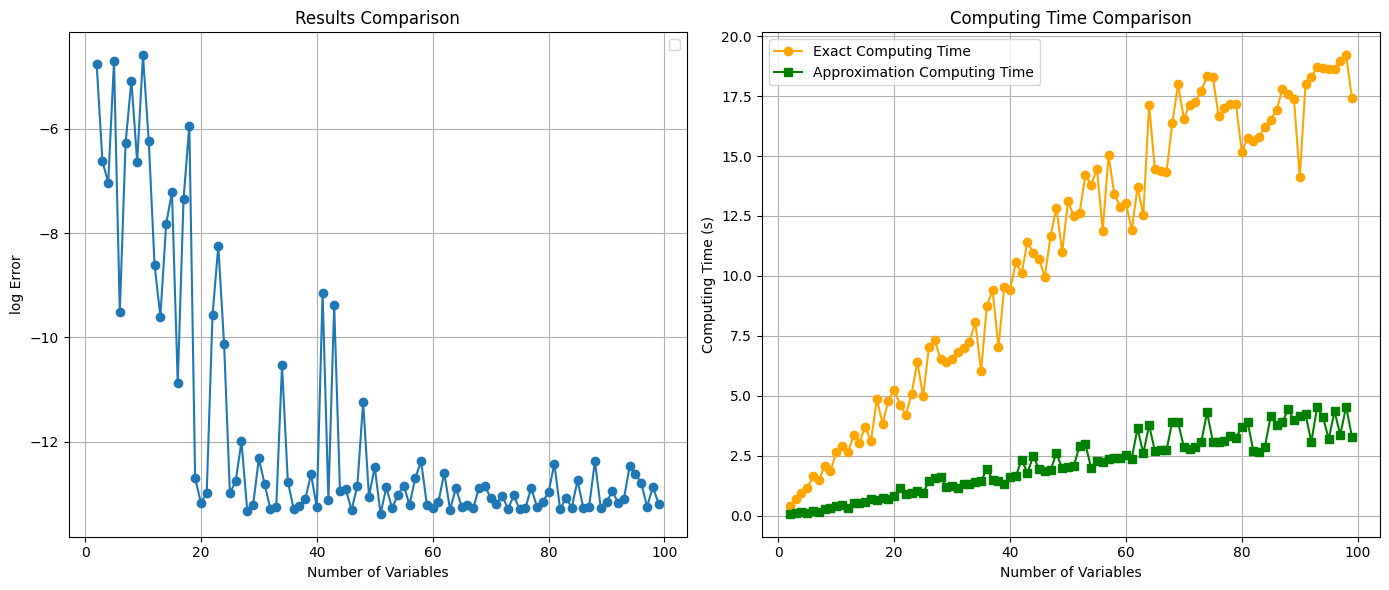
\includegraphics[width=\textwidth]{../../code/notebooks/images/comparison.png} % Replace with your image filename
	\caption{Max and BoostMax comparison}
	\label{plot}
\end{figure*}


\subsubsection{Upper bound}
For large values of \( y \), the factors in the product \( F_Y(y) \) tend to 1, while the PDF inside the summation approaches 0. Consequently, the summation result tends to 0. In general, for a Gaussian distribution \( N(\mu, \sigma) \), the following holds:
$$P(X > \mu + C \sigma) = 0.0015$$
for \( C = 3 \).

To improve the approximation of the upper bound, a larger value of \( C \) (e.g., \( C = 5 \)) is selected. This choice significantly reduces the probability, yielding a more reliable approximation. The upper bound is then given by:
$$UB = \max_{i=1, \ldots, n} \{\mu_i + 5 \sigma_i\}$$
The max operator is used to ensure that the upper bound founded is valid for all the random variables $X_1, X_2, ..., X_n$. For even larger values of \( C \), it is possible to compute a wider upper bound, allowing for a better approximation of the expected value. However, this comes at the cost of increased computational time.

\subsection{Asymptotic approximation}
Since computing the exact method can require a significant amount of time for a large number of random variables, an approximation method based on extreme value theory was studied.
\textbf{Theorem (H., Jagers, Sudbury \& Tokarev, 2009) \cite{hamza2009mixing}}: Let $X_1, \ldots, X_n$ be independent random variables and let $E[X_i^j]$ the $j-th$ moment of the random variable $X_i$. Define $M_j = \mathbb{E}[\max\{X_1^j, \ldots, X_n^j\}]$ for $j = 1, 2, \ldots, n$, then 
\begin{align*}
    \frac{1}{n} \sum_{j=1}^n M_j &\leq \mathbb{E}[\max\{X_1, \ldots, X_n\}] \\
    &\leq \frac{1}{n} \sum_{j=1}^n M_j + \frac{n-1}{n} \cdot \\ 
    & \qquad \qquad \cdot \max\{M_1, \ldots, M_n\}
\end{align*}

The theorem provides insightful lower and upper bounds, though they become challenging to compute for a large number of variables. The main idea was to use Fréchet, Weibull or Gumbell distribution to model $Y$ according to the \textit{Fisher–Tippett–Gnedenko theorem} \cite{fisher1928limiting} that was originally defined for iid random variables but more recent studies show a similar application for the not iid case. Authors in \cite{padua2013distribution} tried to approximate $Y \dot \sim \ G(\alpha, \beta)$ fixing the number of means and variances and then increasing the number of observations $N$ for each component distribution function. As the number $N \rightarrow \infty$, authors applied the stability postulate in order to find the parameters $\alpha$ and $\beta$.

%\begin{align*}
%	\alpha = \frac{1}{n} \sum_{i}^n{\mu_i} + \frac{h(0)}{\sqrt{n}} %\sqrt{\sum_{i}^n{\sigma_i^2}} 
%\end{align*}

%\begin{align*}
%	\beta = \frac{1}{\sqrt{n}} \sqrt{\sum_{i}^n{\sigma_i^2}} \theta 	
%\end{align*}

%where $h(0) = \ln(-\ln(G(0)))$ and 

So, we can define easily the expected value of the maximum as follow
\begin{align*}
	\mathbb{E}[Y] = \alpha + \gamma \beta
\end{align*}
where $\gamma \approx 0.57721$ is the \textit{Euler–Mascheroni} constant. Nevertheless, in our opinion, the paper lacks certain concepts, and therefore, further work and study are needed to develop a more robust solution for the asymptotic results.
